\section{Introduction}\label{sec::introduction}
\subsection{Motivation}
% Overall context
Ever growing amounts of data require effective and efficient storage solutions as well as highly scalable, interactive methods to gain new insights through exploratory analysis or to prove assumptions. Almost all data is subject to change. Nowadays storage is cheap and adheres to Moore's law\cite{MOORE} of doubling about every 18 months supporting the storage of several snapshots of time varying data. Furthermore existing storage techniques minimize the impact of storing such potentially very large data-sets.

Hierarichal information is inherent to many datasets. It is almost always mapped through primary-/foreign-key relations in relational databases. Whereas this might be sufficient in many situations it introduces an additional artificial mapping. Using either a graph-DBMS for directed acyclic graphs (DAG)s or a native XML-DBMS for tree-structures facilitates a straight forward approach of storing data as well as efficient traversal methods and other domain specific advantages (for instance Dijkstra's algorithm for shortest path search in graph databases and most often extensive XQuery support in XML-DBMS). Our aim is to compare tree-structures, 

\emph{Treetank} is a DBMS which offers effective and efficient storage of temporal tree-structures and is developed in the \emph{Distributed Systems Group} at the \emph{University of Konstanz}. While it has been developed from scratch as a persistent, secure storage, revisioning is one of it's core aspects. Several well known revisioning/backup strategies are adapted and implemented. Treetank supports full, incremental and differential revisioning. Furthermore a novel approach called sliding snapshot achieves a good balance between the deficiencies of these techniques and stresses their advantages \cite{TREETANK}.

\subsection{Problem Statement}\label{subsec::problem}
% Problem statement
Todays challenges in database research includes the analysis of increasingly large amounts of data. Storing not only one version of a tree-structure but several similar versions proves this task. Analysts typically face the problem of quickly gaining knowledge from a database with potentially large amounts of uninteresting data for the task at hand. They literally have to find a needle in a haystack, which is commonly known as the "information overload" problem. While coping with rapidly increasing amounts of data is effectively solved by means of Treetank, comparing the tree-structures requires sophisticated methods on top of it. 

Generally two cases for comparing tree-structures have to be distinguished.

\begin{itemize}
\item Tree-structures evolving naturally through applying changes. Snapshots of these tree-structures are either imported through iteratively calculating structural differences between a new snapshot and the last stored revision in Treetank or changes are applied directly using the Java-API offered by Treetank. Each snapshot is stored as a subsequent revision.
\item Tree-structures which are derived from a base version but have changed independently. The base version is either programatically build using the Java-API or through the import of an XML-document. Other tree-structures are created by first reverting to the base revision and either applying changed directly through Treetank's Java-API or comparing another similar tree-structure to the base version utilizing an ID-less diff-import algorithm which first matches nodes based on predefined similarity measures and then applies edit-operations to derive the tree-structure.
\end{itemize}

Both cases eventuate in storing a temporal tree-structure in Treetank either based on applying changes to the last stored revision (the first case) or to the first revision (the second case).

The research task adressed in this thesis is defined as:

\begin{mydef}
Provide methods to help analysts to quickly gain knowledge from comparing tree-structures.
\end{mydef}

\subsection{Approach}
% Approach
A promising solution to the task at hand is to use methods from "Visual Analytics", a term coined by James J. Thomas in \cite{VISUAL_ANALYTICS}. Thomas states that Visual Analytics is "the science of analytical reasoning facilitated by visual interactive interfaces.". Thus we aim to provide (at least semi-)automatic analytical methods facilitated by an interactive visual interface. Analytical methods are inevitable to compare several revisions of a tree as well as the similarity of node kinds based on predefined measures. Furthermore interesting patterns can be revealed by custom \texttt{XPath} queries. Treetank is used to handle large tree-structures.

Whereas hierarichal visualizations have been studied for some time and sophisticated representations have been found, Visual Analytics of comparing tree-structures just recently gained momentum. 

\subsubsection{Value of visualizations}
Francis J. Anscombe reveals the value of graphs (which is generalizable to every (useful) kind of data-visualization) by illustrating in a simple example with four data sets, why graphs are essential to good (statistical) analysis. Using statistical calculations from a typical regression program shows that each computation yields the same result even though fundamental differences are visible on first glance once plotted. Furthermore human brains are trained to interpret visual instead of textual content which is another facet illustrated by this example. It's almost impossible to gain further insights running through the printed out form of these data sets \cite{ANSCOMBE}. 

\subsubsection{Comparison of tree-structures}
In order to be human readable every tree-structure has to be serialized in some form. Character based line by line comparsion difference-tools as for instance used within Subversion (SVN) or the GNU diff tool to compare serialized textual tree-structure representations most often %makes little to no sense. 
doesn't add up. Even though most of them colorize the differences based on character differences or provide other limited graphical representations of the differences encountered they can't recognize the tree-structure and certain domain specific characteristics. For instance XML (Extensible Markup Language), which is a human readable meta markup language and used to import data in Treetank, exemplary for tree-structures in general, has some inherent features which can't be recognized by such tools. Among those are the \emph{lack of semantic differences} in case two XML documents only differ by an arbitrary amount of whitespace between attributes, namespaces\footnote{special kind of attributes} and elements or the permutation of attributes. Changes from empty elements to start tag, end tag sequences (\texttt{<root/>} to \texttt{<root></root>}) or inversely must not be considered as well. Furthermore moves of nodes or subtrees and differences in the order of child nodes can't be determined. The major disadvantage however attributes to the tree-structure itself. Node-boundaries can't be recognized as these tools incorporate no knowledge about the structure itself. A diff between two very simple XML documents (or two versions thereof) done with GVim, which utilizes a line by line character based comparison algorithm is illustrated in figure \ref{fig:faileddiff}. Several of the aforementioned deficiencies can be easily spotted in this simple example. 

\begin{figure}[tb]
\center{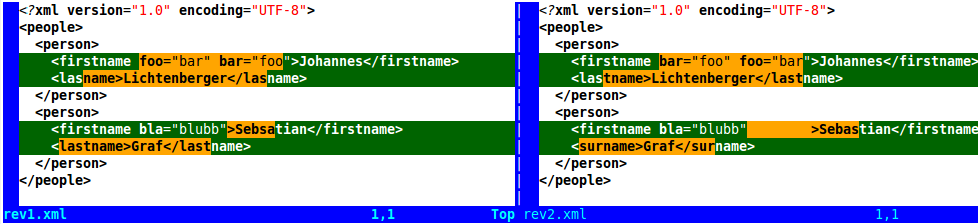
\includegraphics[width=\textwidth]
{figures/gvimdiff.png}}
\caption{\label{fig:faileddiff} Diff example illustrating the deficiencies of line by line character based diff tools}
\end{figure}

While several data mining tools are available which specify on specific tasks, XML is in fact a semi structured, flexible, meta markup language. XML in stark contrast to relational data does not have to adhere to a schema or structure, which has to be planned and implemented beforehand. Due to that it is mandatory that the visual interface offers great flexibility and thus isn't restricted to a special use case.

Thus the high level goal defined in the last section (\ref{subsec::problem}) can be divided into:
\begin{itemize}
\item Preprocessing and import of data.
\item Structural comparison based on \texttt{insert-/delete-}operations.
\item Comparison of non-structural data (for instance \texttt{TextNode} values).
\item Extend with \texttt{replace}, \texttt{update} and \texttt{move}-operations (optional).
\item Provide visualizations to quickly gain insights into which subtrees/nodes have been changed.
\end{itemize}

\subsection{Application domains}

Motivating examples are manyfold. To meantion just a few of them:

\begin{itemize}
\item Even though companies and the relationship among employees in general form a directed acyclic graph (DAG) most of them are organized in a hierarichal tree-structure \footnote{also referred to as a connected acyclic graph (CAG)} which evolves over time. Appropriate representations of the changes enables to track the career of certain persons or might reveal how sub-organizations are evolving very well while others might not due to the success or failure of products.
\item The hierarichal structure of filesystems and the recently upcoming abilities to store Snapshots, which is based on the COW (copy-on-write) implementation of recent filesystems as for instance BtrFS and ZFS. Users might want to quickly determine when and where directories/files have been moved, when they have been deleted or created and so forth. An example application which recently reached end users through Apples' OS X is TimeMachine. Furthermore permission rights, file-extensions and hash-values of files can be tracked through time, which might be of great value to security engineers.
\item Humans which are interested in detailled changes of several versions of some products and compare their attributes and features. This analysis might even reveal how companies prioritise the development and enhancement of certain features.
\item Tracking changes in software development based on a low level Abstract Syntax Tree (AST) comparsion \cite{telea2008code}. This might reveal code splits, merges, deletions and inserts. At a greater scale constant unmodified code can be tracked through several revisions revealing stable code in contrast to recently introduced new features. The latter usually is subject to many changes.
\item Biologists have to understand structural differences of phylogenetic/evolutionary trees \cite{munzner2003treejuxtaposer} which in general can be very large. An efficient comparsion algorithm is needed as well as some kind of visual interface to asses biologists in locating and exploring tree differences. Juxtaposer is going to be described in greater detail in the next chapter.
\end{itemize} 

\subsection{Contributions}
Treetank offers great storage benefits regarding revisioning. However it lacks support of analytical methods for the detection of differences between these revisions and visualizations thereof. Thus the main aim of this thesis is the research and development of an interactive visual interface supporting analysts to determine changes in temporal hierarichal tree-structured along analytical methods to compute the differences.

In a nutshell this thesis provides the following computer science contributions:

\begin{itemize}
\item Preprocessing of realworld XML data, for instance the import of \emph{Wikipedia} and monitoring changes in a specific Filesystem directory.
\item Several contributions to our backend, Treetank including compacting the storage and new edit-operations to support the implementation of an ID-based differencing algorithm and expressive visualizations. Furthermore a new subtree-insertion operation based on a existing component in Treetank speeds up hashing of subtrees considerably from $O(n^2)$ to $O(n)$ due to a simple postprocessing postorder traversal whereas $n$ is the size of the nodes in the inserted subtree.
\item Analytical methods (algorithms) to compute structural and non structural differences between similar or evolving tree-structures.
\item A \texttt{TextView} which serializes an aggregated tree-structure to a syntax highlighted XML output. Furthermore only the visible area plus additionally space to add a slider is filled.
\item A \texttt{SunburstView} facilitating comparison of tree-structures by a novel layout algorithm and several pruning techniques.
\item A \texttt{SmallmultipleView} supporting different modes (incremental, differential, a hybrid mode and sorted by similarity).
\item Interaction mechanisms like zooming/panning, a fisheye view, pruning, support of XPath-queries and several other techniques.
\end{itemize}

\subsection{Conventions}
Pseudocode which is used to illustrate algorithms in this thesis is based on a Java-like syntax as our prototype is based on Java, that we assume familiarity with a C-like syntax (as Java's) and that we want to reduce common errors which most probably arise once describing algorithms in terms of very abstract pseudocode. A paper reviewed during the implementation of our prototype contained errors in the pseudocode that might have been circumvented if stuck to a more precise description of the implementation. Similarly, the devil is in the detail. On the far side of most Java-specific details are omitted, which would otherwise introduce a lot of complexity to the pseudocode resulting in little to no value for the algorithm described. The following conventions in particular apply:

\begin{itemize}
\item The logical operator \emph{$||$} from Java and other programming languages is denoted by \emph{OR}.
\item Similar the logical operator \emph{$\&\&$} is denoted by \emph{AND}.
\item Variable or reference assignments \emph{$=$} are denoted by \emph{$\leftarrow$}.
\end{itemize}

\subsection{Outline}

The work is structured as follows:

\begin{description}
\item[Chapter 2] provides an overview of algorithms to compute differences in tree-structures. Next, research efforts in visualizing differences of trees are examined. The chapter concludes with a summary of the visualizations which are examined in respect to various attributes.
\item[Chapter 3] starts off with a short description of Treetank and its encoding. Next, as most tree-structures do not use unique node-IDs we compute differences based on the FMSE-algorithm. FMSE tries to match nodes based on similarity measures for leaf- and inner-nodes in the first place and in subsequent steps modifies a tree with as few edit-operations as possible to transform the first tree into the second tree. Thus implementation of FMSE is described as well as numerous extensions to Treetank to support the implementation. Once the data is imported we use an internal diff-algorithm based on unique node identifiers to compare several trees, which is described thereafter. The chapter concludes with performance measures of our ID-based algorithm and concludes with a short summary.
\item[Chapter 4] is introduced with an overview of the GUI structure. Detailed descriptions of our visualizations follow. Furthermore several interaction mechanisms are examined.
\item[Chapter 5] demonstrates the feasability of our approaches based on real world data.
\item[Chapter 6] discusses our approach in relation to the State-of-the-Art.
\item[Chapter 7] summarizes the results and provides suggestions for future work.
\end{description}


